Software testing is a crucial aspect in software development, ensuring
that applications function correctly, meet requirements, and provide a
reliable and secure user experience. Among various testing methods,
{\bf fuzz testing} (or {\bf fuzzing}) involves providing random or
semi-random data inputs to a program in an attempt to trigger
unforeseen behaviors, crashes, or security flaws. Unlike traditional
testing methods that rely on predefined inputs, fuzz testing involves
automatically generating a wide range of random, unexpected, or
malformed inputs to the system under test. This approach is invaluable
for uncovering obscure bugs and security flaws that might be missed by
other testing strategies. By exposing software to a diverse set of
inputs, fuzz testing can reveal how the application handles unexpected
conditions, thus identifying potential points of failure or security
vulnerabilities. This is particularly important for security-sensitive
applications where robustness against unusual or malicious inputs is
essential.

%Overall, fuzz testing enhances the reliability and security of software by proactively identifying and addressing issues that could lead to crashes, data corruption, or breaches.

Among fuzzing methods, a {\em coverage-guided fuzz testing framework}
is a systematic approach to identifying software defects or
vulnerabilities through automated
testing. Figure~\ref{fig:coverage-fuzz} illustrates its process. The
first stage, which is the {\em seed corpus generation}, starts with
creating an initial set of test cases, known as the seed~corpus. These
test cases are typically generated manually or extracted from existing
test suites, real-world inputs, or example code snippets. Through a
selection, each test case in the seed corpus is chosen for the second
stage: {\em fuzzing input generation}. In this stage, the fuzzing
engine generates a large number of mutated or random inputs based on
the seed corpus. These inputs are designed to explore various paths
and edge cases within the target program under test. In the third
stage, {\em target program execution}, the generated inputs are fed
into the target program. It executes the inputs and processes them
according to its normal operation. During this stage, the framework
{\em monitors code coverage}, tracking which parts of the target
source code are exercised by the inputs. This is typically done using
instrumentation techniques or by analyzing execution traces. During
execution, if the execution of an input triggers an unexpected
behavior, e.g., a crash, assertion failure, or memory corruption, the
framework identifies it as a potential defect. The detected faults are
logged and reported to developers for further investigation
and~resolution.

In the next stage ({\em feedback loop}), the framework selects the
best test cases with highest code coverages and adds them back to the
seed corpus/pool. The framework continuously mutates and generates new
inputs based on the coverage feedback and best test cases received
for the target program. The inputs that explore previously untested
paths or trigger new code coverage are prioritized for further
mutation and testing. The fuzzing process iterates continuously,
generating new inputs, executing them against the target program, and
refining the test cases based on the coverage feedback. As the process
progresses, the framework may analyze and prioritize inputs based on
factors such as code coverage, execution time, and the severity of
detected faults. This helps focus testing efforts on the most
promising areas of the codebase.

Despite its popularity and successes, the coverage-guided fuzzing
framework still has the following key shortcomings. First, the
framework might suffer the issue of inefficiency and high resource
consumption: it generates a large number of test cases without prior
knowledge of their code coverage quality. This can lead to inefficient
resource and time usage, as a significant portion of the generated
test cases might have lower coverage, consuming computational
resources without contributing meaningfully to the identification of
new code paths or defects. Second, it has an ineffective feedback
loop: since the framework relies solely on actual execution during the
target program's runtime to determine test case quality (in terms of
code coverage), there's a risk that a large number of generated test
cases might be executed without contributing much value to
the feedback loop. This hinders the effectiveness of the iterative
fuzzing process in terms of enhancing the seed corpus with
high-quality test cases. Moreover, it is challenging to produce better
seeds: determining which test cases should be added to the seed corpus
for future iterations becomes challenging when the primary mechanism
for inclusion is from actual execution during fault detection. The
lack of a proactive strategy for identifying and prioritizing
high-quality seeds can hinder the evolution of the seed corpus and
make the process stuck in the plateau where coverage is not
improved~\cite{gao2023beyond}.

\begin{figure}[t]
    \centering
    \begin{minipage}{0.5\textwidth}
        \centering
        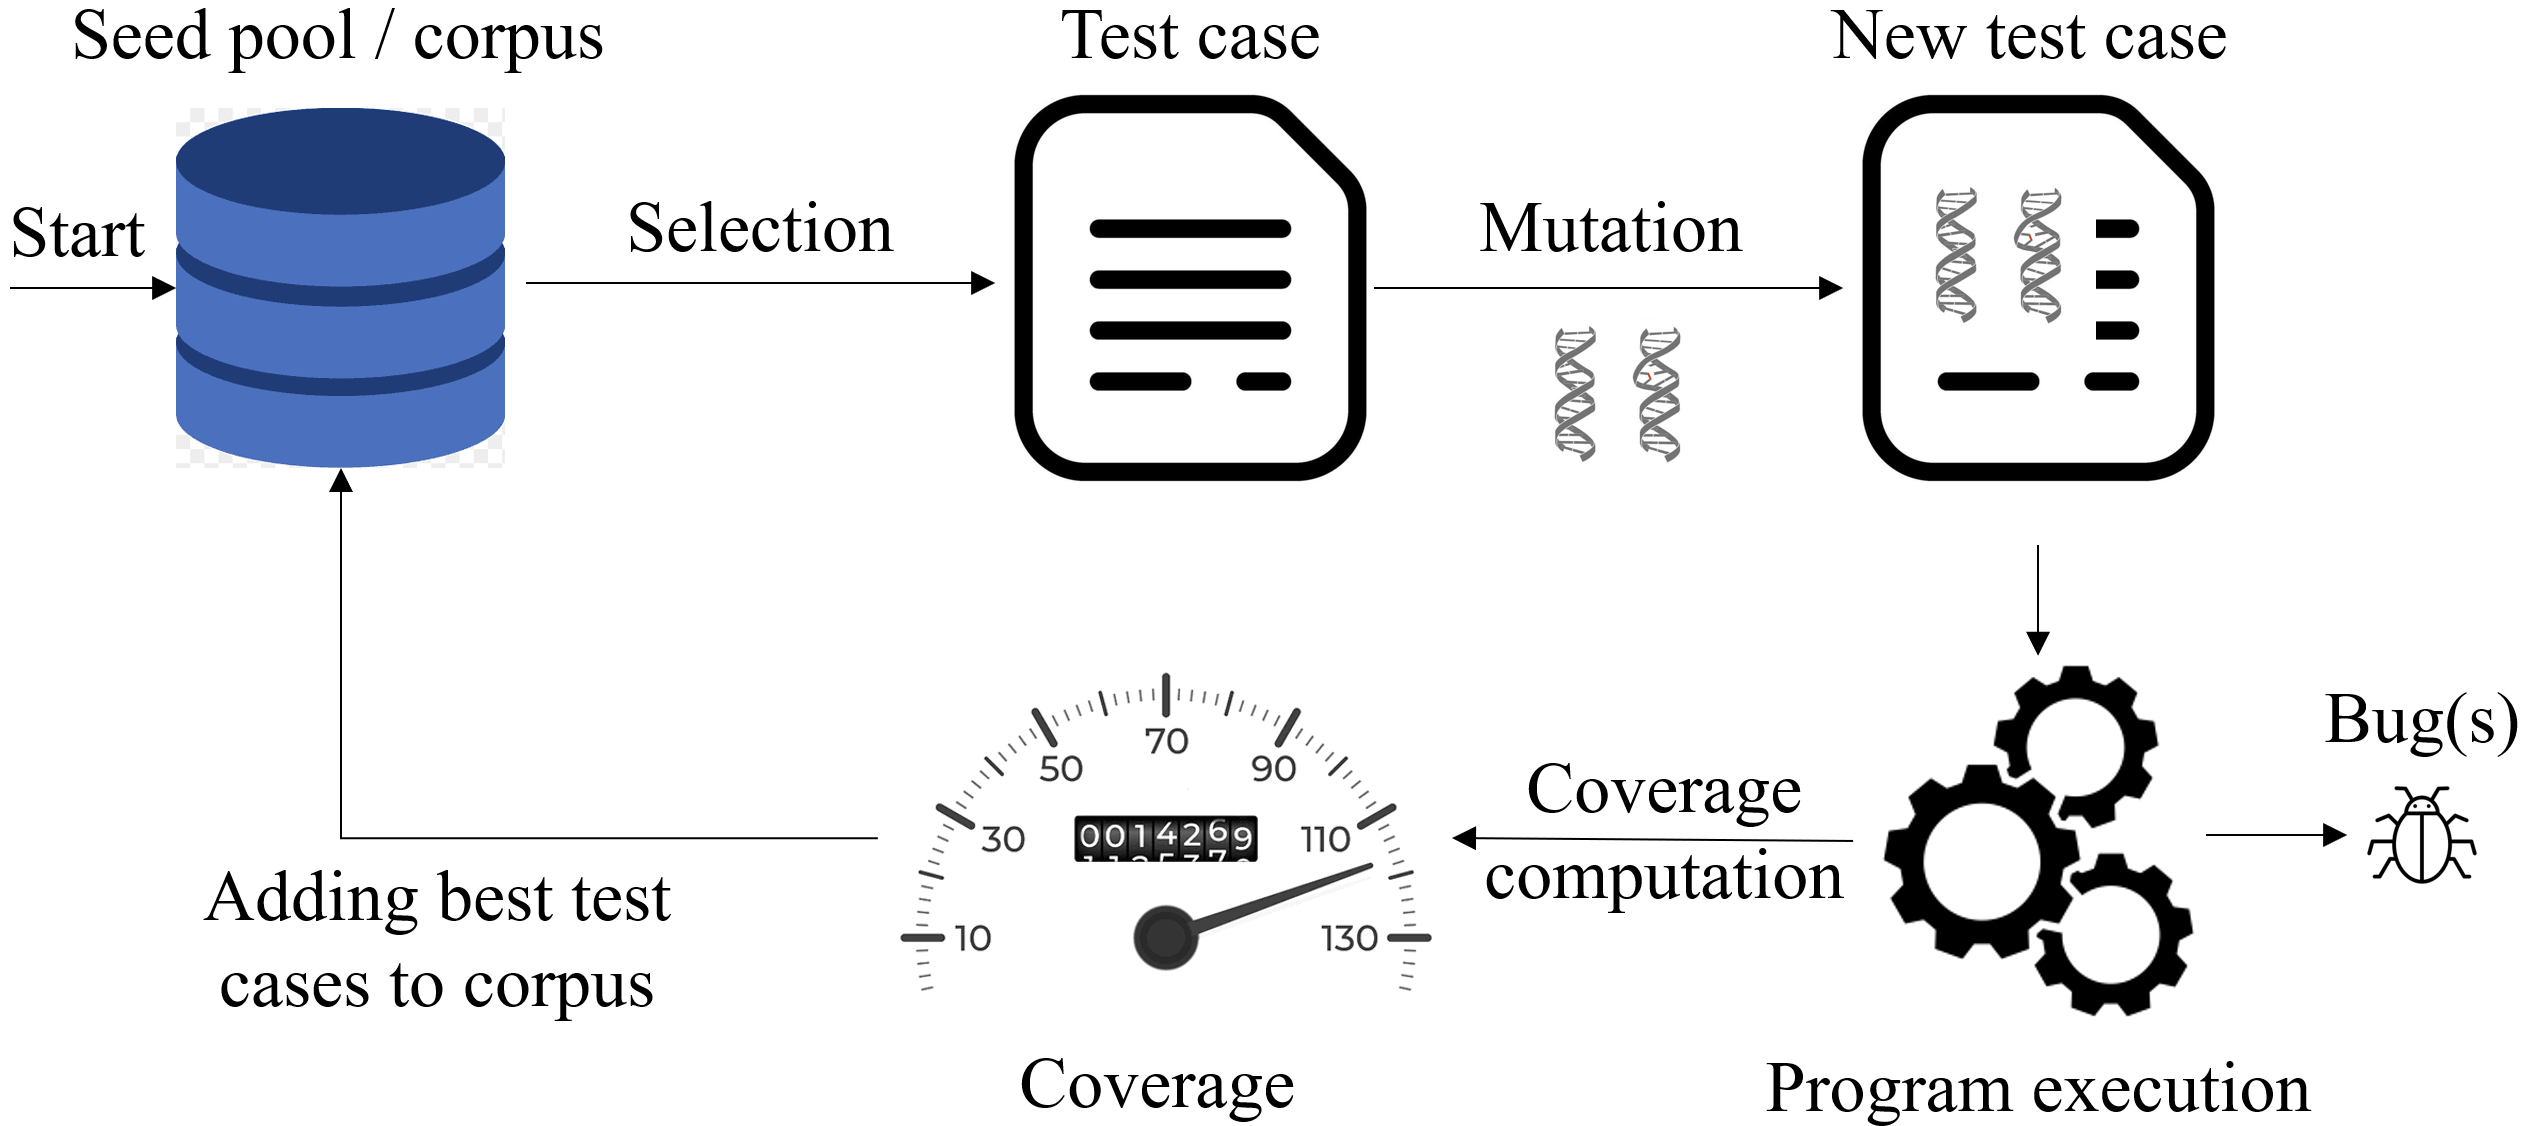
\includegraphics[width=3.25in]{coverage-fuzz.png}
        \vspace{-18pt}
        \caption{Traditional Coverage-Guided Fuzz Testing}
        \label{fig:coverage-fuzz}
    \end{minipage}%
    \begin{minipage}{0.5\textwidth}
        \centering
        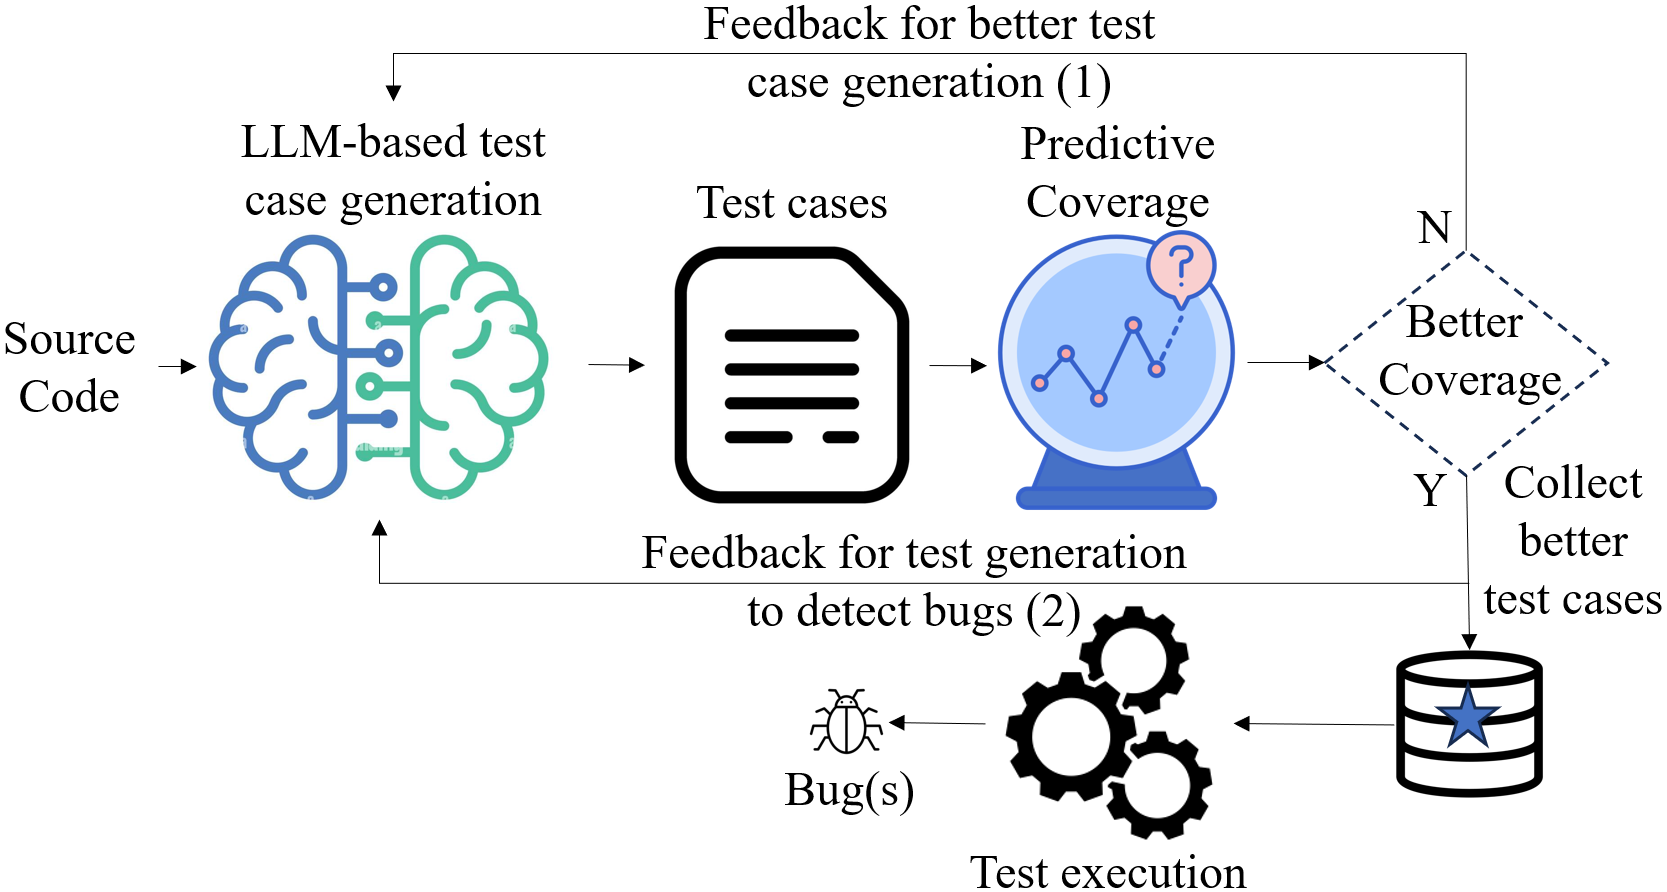
\includegraphics[width=3.3in]{fuzzwise2.png}
        \vspace{-18pt}
        \caption{Predictive Coverage-Guided Intelligent Fuzzing}
        \label{fig:fuzzwise}
    \end{minipage}
\end{figure}

%\begin{figure}[t]
%\begin{center}
%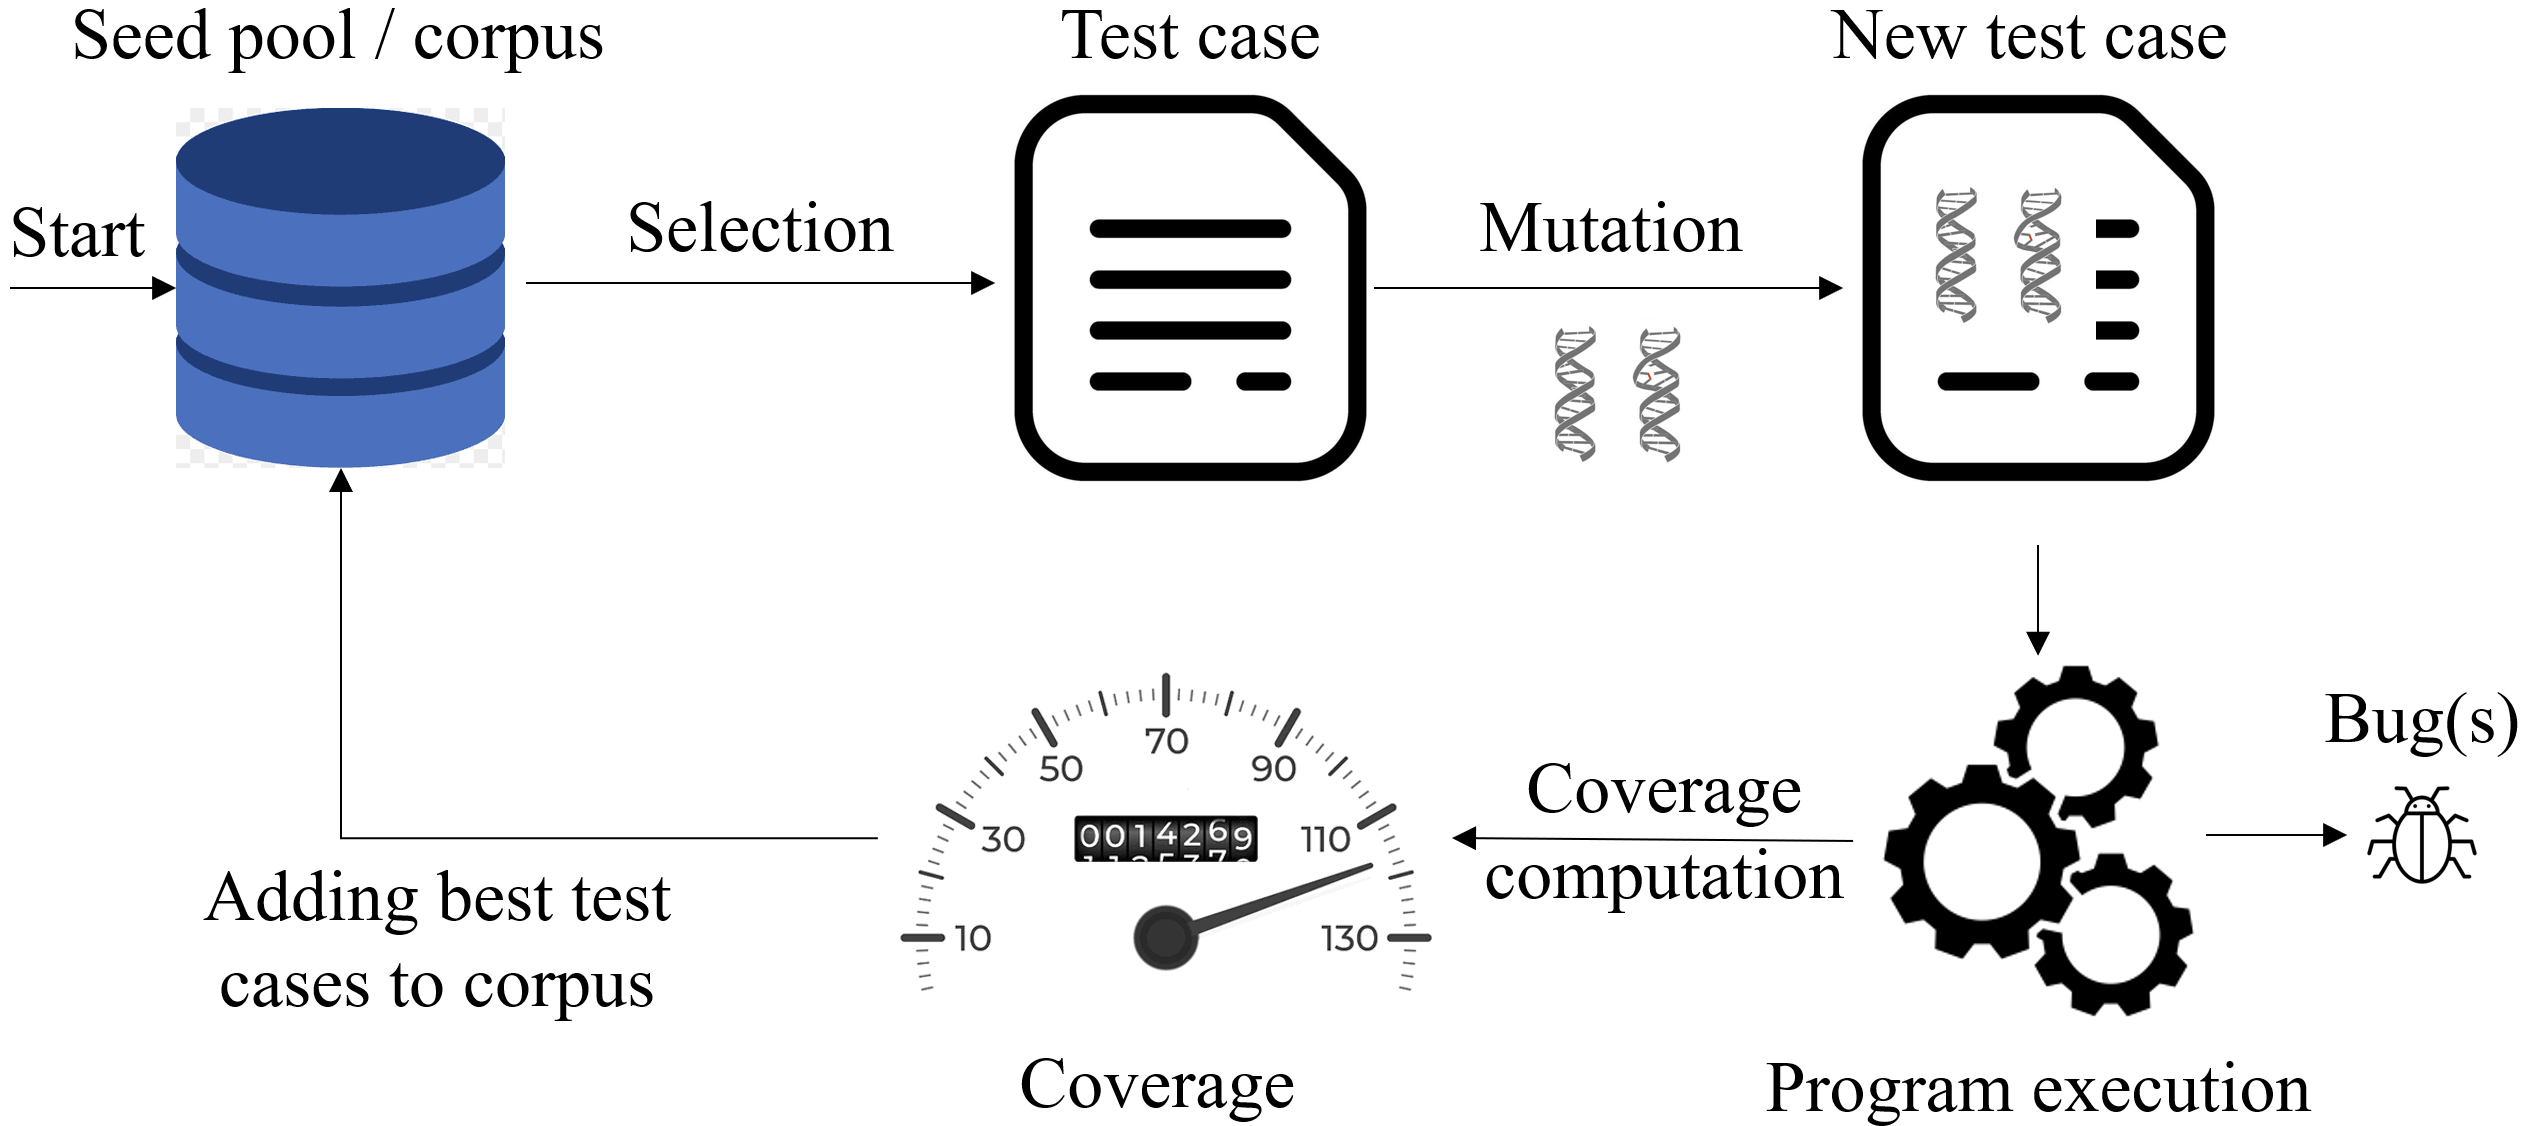
\includegraphics[width=3.4in]{coverage-fuzz.png}
%\vspace{-6pt}  
%\caption{Predictive Coverage-Guided Intelligent Fuzzing Framework}
%\label{fig:coverage-fuzz}
%\end{center}
%\end{figure}

%\begin{figure}[t]
%\begin{center}
%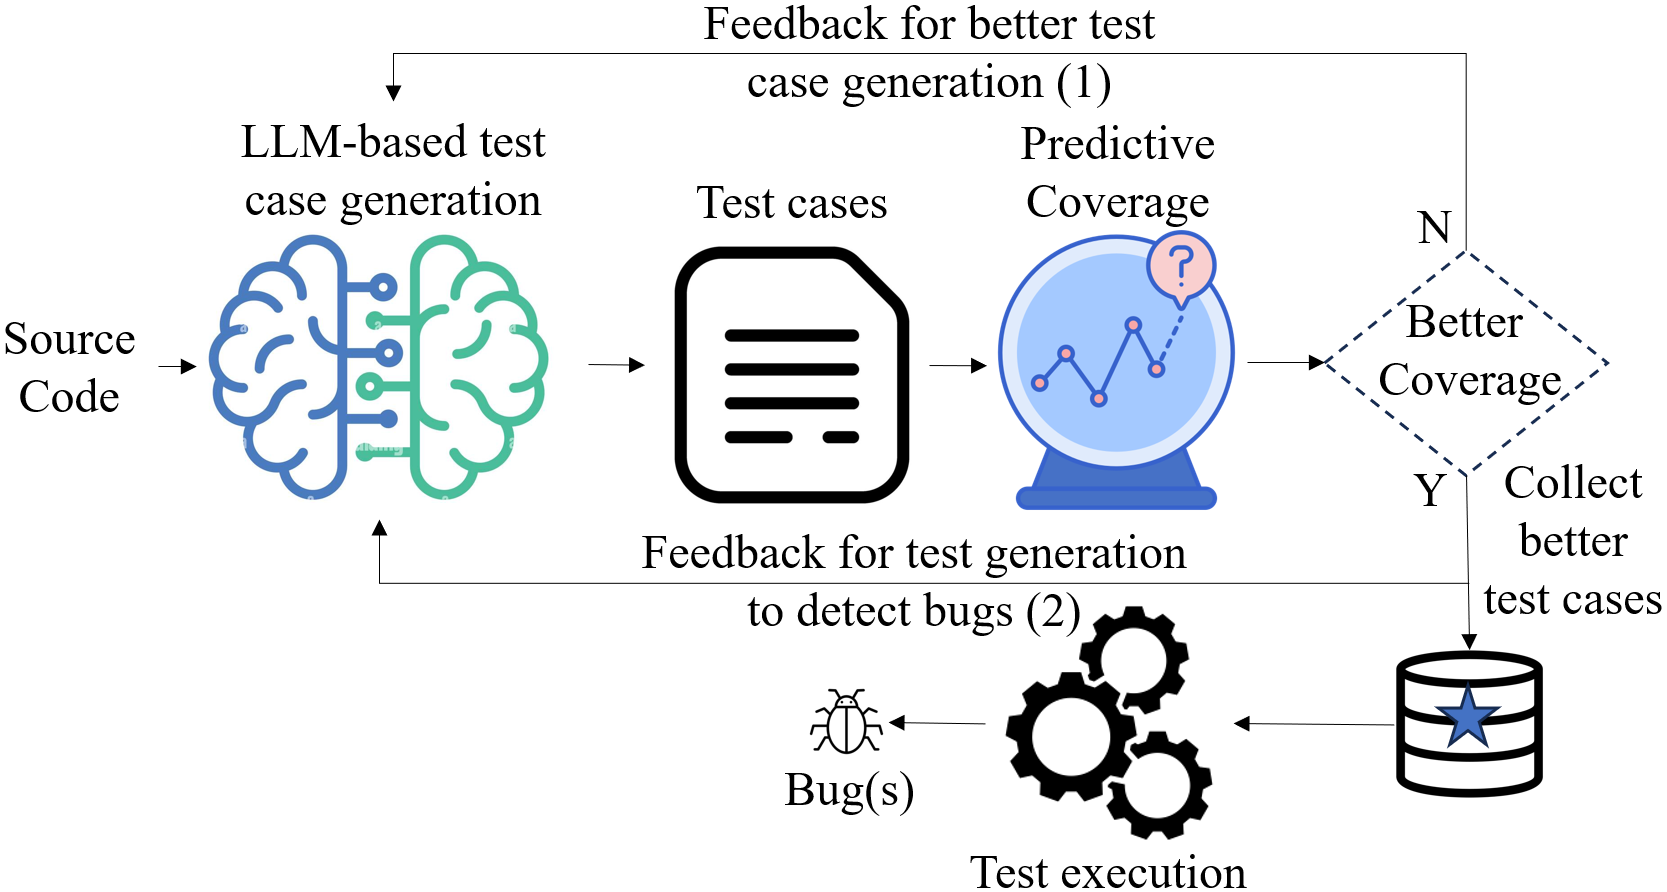
\includegraphics[width=3.5in]{fuzzwise2.png}
%\vspace{-15pt}
%\caption{Predictive Coverage-Guided Fuzzing Framework}
%\label{fig:fuzzwise}
%\end{center}
%\end{figure}

\subsection{Predictive Coverage-Guided Fuzzing Framework}

In this work, we propose {\tool}, a predictive code coverage-guided
intelligent fuzzing framework without actual test execution
(Figure~\ref{fig:fuzzwise}). For an upfront test quality assessment,
our \underline{first idea} is to develop a Large Language Model (LLM)-based code
coverage prediction approach, CodePilot~\cite{forge24}, that estimates
the quality of the generated test cases with regard to their code
coverages. The preliminary work on code coverage prediction is
described in~\cite{forge24}. This predictive approach aims to
identify, prioritize, and execute only the test cases that are likely
to contribute to higher total code coverage, thereby conserving
computational resources in actual execution, and focusing testing time
on the areas that likely need further testing.

Our \underline{second fundamental concept} aims to tackle the challenges
associated with mutations and the seed corpus. Instead of relying on
the conventional approach of mutating tests and enhancing the seed
corpus, we propose leveraging a LLM to automatically generate test
cases for the given source code under test. Within {\tool}, the
feedback loop is activated subsequent to the prediction of code
coverage. Once our predictive code coverage module determines that a
generated test case does not contribute to a higher total coverage of
the current test suite, we reintroduce these cases to the LLM.
This process enhances the generation of test cases from the LLM with
the goal of covering more un-tested areas in subsequent cycles. This
is carried out in the feedback loop (1) (Figure~\ref{fig:fuzzwise}).

Once predictive code coverage module determines that~a generated
test case would contribute to achieving higher overall coverage, we
collect it into the current test suite. However, we defer their
execution at this stage. Instead, the framework proceeds to the second
loop (2), where it prompts the LLM to generate additional test cases
with the main goal of enhancing the probabilities of detecting bugs and
runtime errors.

To enhance both effectiveness and efficiency, we instruct the LLM to
generate multiple test cases simultaneously: one seed test case and
several ``close'' variants. This approach aims to exploit a
faulty area within the source code by producing test cases closely
related to the seed. As the second loop (2) starts, we
expect that the LLM will begin exploring a new faulty area in the
source code. This functionality mirrors the traditional approach of
using different seed test cases. By adopting this strategy, we aim to
address the ``plateau'' issue, where the fuzzing process becomes
stagnant despite generating numerous mutations. The process will
terminate once either the cumulative code coverage of the entire test
suite reaches 100\% or the predetermined time limit is reached.


%We have conducted several experiments to evaluate {\tool}. Our result
%in the FixEval dataset~\cite{haque2023fixeval} shows that within a
%time limit, {\tool} generates significantly less test cases (only
%about 0.0065\%), yet to detect more runtime errors than the
%conventional fuzz testing framework in Jazzer~\cite{jazzer}. {\tool}
%is more efficient in runtime error detection compared to the baseline:
%on average, {\tool} executed {\bf 163} generated test cases to detect a
%runtime error, while Jazzer executed {\bf 4,217,067} test cases per error,
%thus showing that {\tool} saves execution time over Jazzer for
%ineffective test cases. The ratio between the number of effective test
%cases over the total number of generated ones for {\tool} ({\bf 0.48})
%is also higher than that of Jazzer ({\bf 0.41}), showing that {\tool}
%produces more effective, higher-quality test cases. Our result also
%shows that it took significantly less number of test cases for {\tool}
%to detect the next runtime error from the previous one than Jazzer.
%Moreover, we show that {\tool} overcomes the coverage plateau better
%than Jazzer. Importantly, the code coverage prediction module is
%sufficiently accurate in which {\bf 67\%} of test cases predicted by
%{\tool} as enhancing the coverage are indeed effective in doing so.

%The key contributions of this paper include:

%{\bf 1. {\tool}:} a novel predictive code coverage-guided fuzz testing
%framework that leverages predictive code coverage to conserve
%computational resouces in execution.

%{\bf 2. LLM-based Test Case Generation:} we leverage LLM to analyze the
%given code and generates the test cases with the feedback loops to
%iteratively improves the test case quality.

%{\bf 3. Extensive Empirical Evaluation:} to demonstrate that {\tool} is
%more effective and efficient than the baseline fuzzing models. Data
%and code is available at~\cite{fuzzwise-website}.







